\section{Resultat}
Denna del av dokumentet presenterar resultatet av vårt arbete.
Här kommer vi diskutera både hur systemet ser ut och används, samt hur
det är uppbyggt rent tekniskt.

\subsection{Översikt av systemet}
Det finns två huvuddelar i systemet. Handböckerna och kartoteket.

Handböckerna beskriver hur man förbereder olika typer av operationer.
Varje handbok har en lista med artiklar som behövs till operationen, en så kallad plocklista.
Artiklarna är kopplade till kartoteket, som bland annat innehåller information om var i förråden artiklarna finns placerade.

När en patient registreras skapas en instans av en handbok.
I denna instans kan man checka av en lista med artiklar som ska användas under operationen och även andra förberedelser.
En samordnare kan se en översikt på hur långt man har kommit med de förberedelserna för varje instans.
Se en översikt i figur \ref{fig:overview}.

\begin{figure}[htbp]
  \centering
  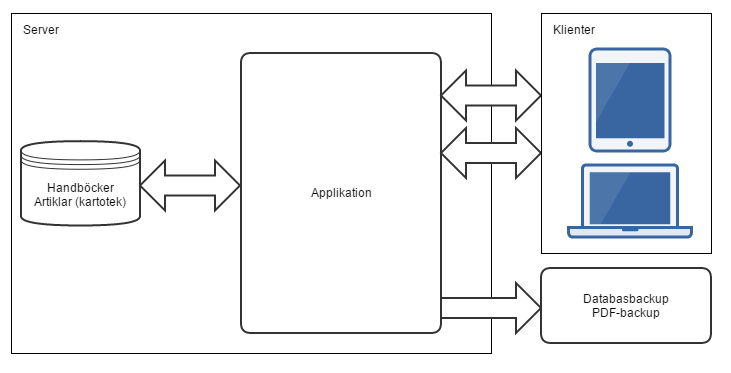
\includegraphics[width=0.9\textwidth]{images/overview.png}
  \caption{Översikt av systemet}
  \label{fig:overview}
\end{figure}

\subsubsection{Server och klient}
Applikationen består av en server som distribuerar en hemsida till flera klienter.
Servern kan köras i en Windowsmiljö.
Hemsidan är responsiv och fungerar på surfplattor och datorer i olika format.

\subsubsection{Kartoteket}
I kartoteket finns information om alla artiklar som Region Östergötland har i förråden.
Här finns bland annat information om var artiklarna är placerade samt information relaterade till inköp av artiklar.

Läs mer om kartoteket i "Kartoteket" nedan.

\subsection{Tekniker}
Vi börjar med att beskriva tekniken bakom systemet.

\subsubsection{Översikt}
Programmet är uppdelat i två delar, en serverdel och en klientdel.
Serverdelen består av databaskopplingar som kopplas ihop och distribueras ut genom hemsidor till klienterna.

\begin{figure}
  \centering
  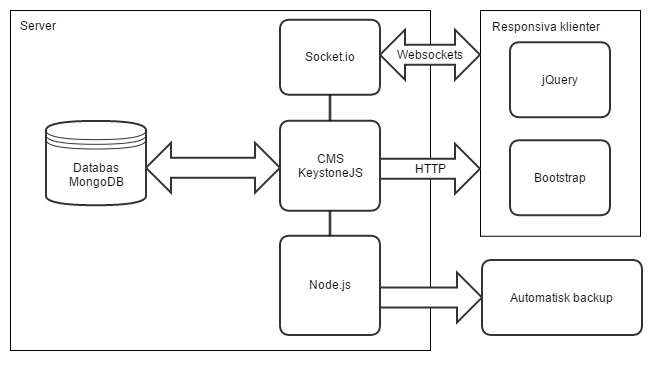
\includegraphics[width=0.9\textwidth]{images/techoverview.png}
  \caption{En översikt över tekniken}
  \label{fig:techoverview}
\end{figure}

I figur \ref{fig:techoverview} kan man se en översikt över de mest betydelsefulla tekniker och bibliotek som används för att bygga upp programmet.

\subsubsection{Back-end}
Koden till servern har skrivits helt i javascript.
Dels för att underlätta inlärningskurvan genom att använda samma språk som på klienten och dels för att realtidskommunikation mellan klienterna underlättas.
Grunden till programmet är node.js vilket är en plattform för att utveckla självständiga program i javascript med inbyggd pakethanterare.
Pakethanteraren gör det enkelt att installera externa bibliotek.

Det största och mest betydelsefulla ramverket för detta projekt är KeystoneJS, ett CMS-ramverk till node.js.
Följande är några punkter KeystoneJS underlättar:
\begin{itemize}
  \item Hjälper till att abstrahera systemet. Se avsnittet om MVC nedan.
  \item Skapar automatiskt en administreringssida för varje databasmodell.
    Huvuddelen av administeringen har dock bytts ut då den automatgenererade kan vara något begränsad.
  \item Har ett inbyggt användarsystem som är lätt att modifiera och byta ut.
  \item Sköter all kommunikation över http-protokollet till klienterna, dvs. gör hemsidan åtkomlig.
  \item Har inbyggt stöd för templatespråk som exempelvis Handlebars\footnote{TODO: bättre referens. http://handlebarsjs.com/ (2015-04-18)} och Less\footnote{TODO: Bättre referens. http://lesscss.org/ (2015-04-18)}.
\end{itemize}

För realtidskommunikation används ett programmeringsinterface vid namn socket.io\footnote{TODO: bättre referens. http://socket.io/ (2015-04-18)} användas.
Det är väldigt smidigt eftersom det väljer automatiskt hur datan ska skickas beroende på vilken webbläsare som används och vad den stödjer.
Socket.io är event-baserat vilket betyder att man skapar events på antingen klient eller serversida som man sedan kan trigga från motsatt sida.
Vanliga javascript-object kan skickas tillsammans med eventen.

\subsubsection{Front-end}
På klientsidan används bootstrap\footnote{TODO: Bättre referens.} och jQuery\footnote{TODO: Bättre referens.}.
Bootstrap har många färdiga CSS-klasser så man behöver inte skriva lika mycket CSS själv.
De klasser som finns är lätta att använda för att skapa responsiva hemsidor.
All kod är dessutom testad för att fungera på olika webbläsare vilket kan vara krångligt att lösa om man skriver all CSS från grunden.
JQuery används för att lättare hämta ut ett element på hemsidan och ändra data i det.
Det finns även många bra jQuery-bibliotek att hämta som gör att man slipper “uppfinna hjulet” i många fall.

För att ytterligare design av hemsidan används LESS\footnote{TODO: Referens.} att användas.
Det är en påbyggnad till CSS som kompilerar till vanliga CSS-filer.
Fördelen med LESS är bland annat att man kan använda variabler och enkla funktioner.
Exempelvis kan variablerna användas för att spara de olika färgerna på hemsidan för att enkelt kunna byta ut dem.


\subsubsection{Struktur}
En nackdel med jQuery gentemot andra bibliotek som exempelvis angular\footnote{TODO: Referens.} är att det lätt blir spaghettikod\footnote{TODO: Måste defineras?}.
För att strukturera så bra som möjligt är det viktigt att koden uppdelad.
För att uppnå detta så kommer varje enskild sida ha minst en skriptfil, en cssfil och en htmlfil.
På vissa sidor är det lätt att det blir stora skript och då bör man dela upp skriptfilen.
Den bästa lösningen är att abstrahera delar av skriptet till egna biblioteksfiler som man kan ladda in och använda.

\subsubsection{Säkerhetskopiering}
Ett system för automatisk säkerhetskopiering i form av en PDF-fil för varje handbok kommer att finnas.
Varje gång en handbok ändras kommer PDF-filen att uppdateras för att matcha handboken.
PDF-filen ska vara utformad så att operationerna kan förberedas utan hjälp från hemsidan.

\subsection{Mekanismer}
Här beskrivs syftet och funktionalitet hos olika delar av produkten.

\subsubsection{Översikt}
Som tidigare nämnts finns en översikt över alla operationsförberedelser.
Denna sida visar alla operationsförberedelser och hur långt är fortskridna.
Här används socket.io för att hela tiden hålla information uppdaterad.

\begin{figure}
  \centering
  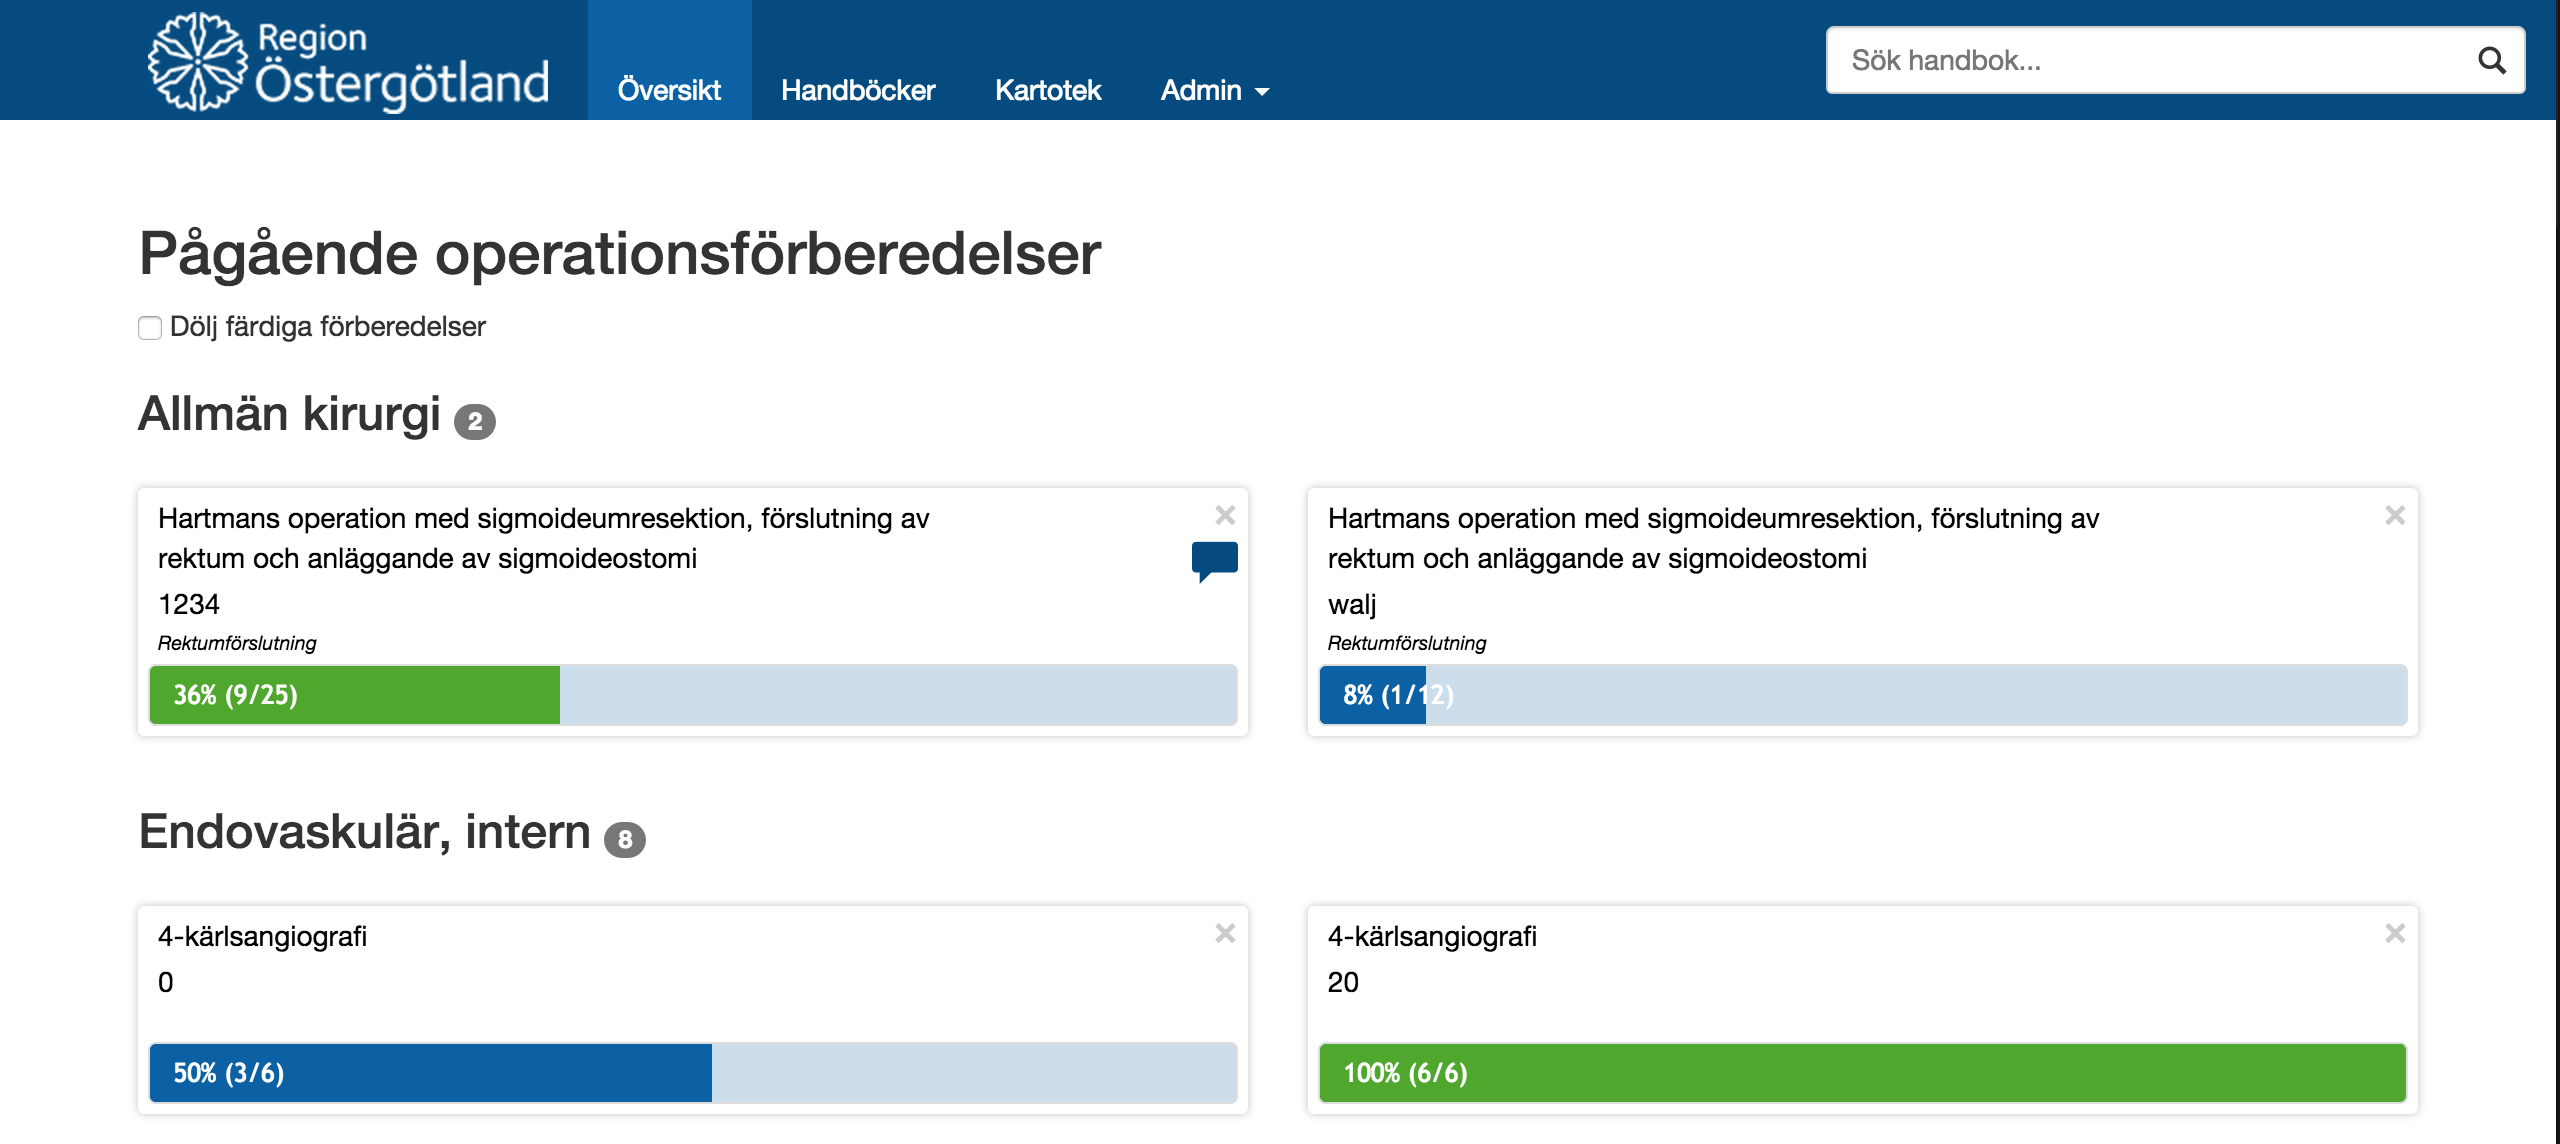
\includegraphics[width=0.6\textwidth]{images/site/overview.png}
  \caption{Bild på översiktsvyn}
  \label{fig:siteoverview}
\end{figure}

I figur \ref{fig:siteoverview} kan man se hur förberedelserna är kategoriserade beroende på vilken kirurgisk specialitet handboken tillhör.
Ibland är det olika samordnare beronde på specialitet och det är då enkelt för en samordnare att hitta de operationerna som personen är ansvarig över.

\subsubsection{Handbok}
En handbok innehåller information om en operationsförberedelse.

\begin{figure}
  \centering
  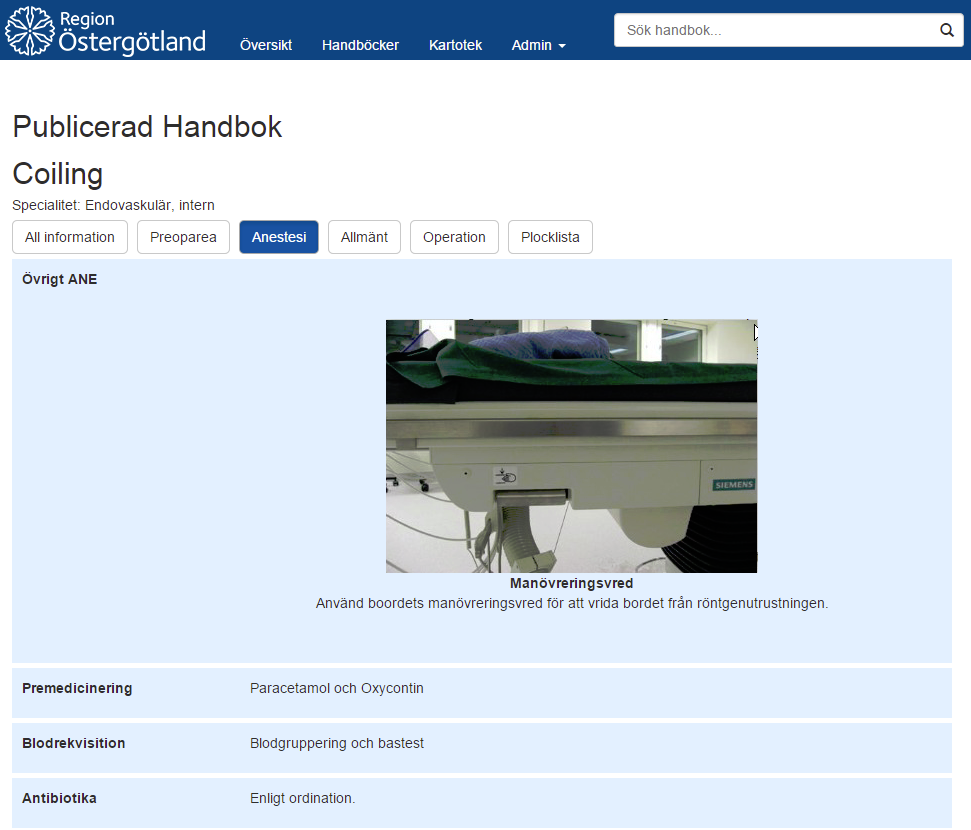
\includegraphics[width=0.6\textwidth]{images/site/handbok.png}
  \caption{En handbok}
  \label{fig:handbok}
\end{figure}

All information i en handbok är uppdelad i olika rubriker. Dessa rubriker kan i sin tur vara uppdelade i olika processer.
I figur \ref{fig:handbok} ser man dels de olika processerna (Preoparea, anestesi, allmänt och operation) samt rubrikerna som hör till processen Anestesi (Övrigt, Premedicinering, blodrekvisition och  antibiotika).
Man kan även se att handböckerna har stöd för bilder.

\subsubsection{Sökfunktion}
Ett krav är att det ska vara lätt att hitta en handbok.
Därför kan man söka både på operationens namn men även på alternativa sökord (taggar), dessa är bra att ha då de medicinska termerna ibland kan vara svåra att komma ihåg.

\begin{figure}
  \centering
  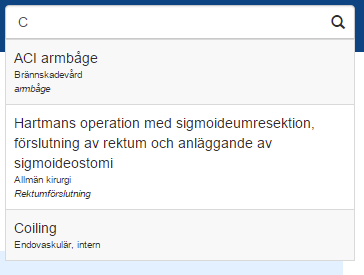
\includegraphics[width=0.6\textwidth]{images/site/search}
  \caption{Sökfunktionen}
  \label{fig:search}
\end{figure}

I figur \ref{fig:search} kan man se sökresultaten där namnet på operationen står i större storlek, och sökorden kursivt i mindre storlek.

\subsubsection{Lista med handböcker}
Applikationen innehåller en enkel lista med alla handböcker.
Den går att sortera på valfri kolumn och kan även gruppera beroende på vilken specialitet handboken tillhör.
Se figur \ref{fig:list}

\begin{figure}
  \centering
  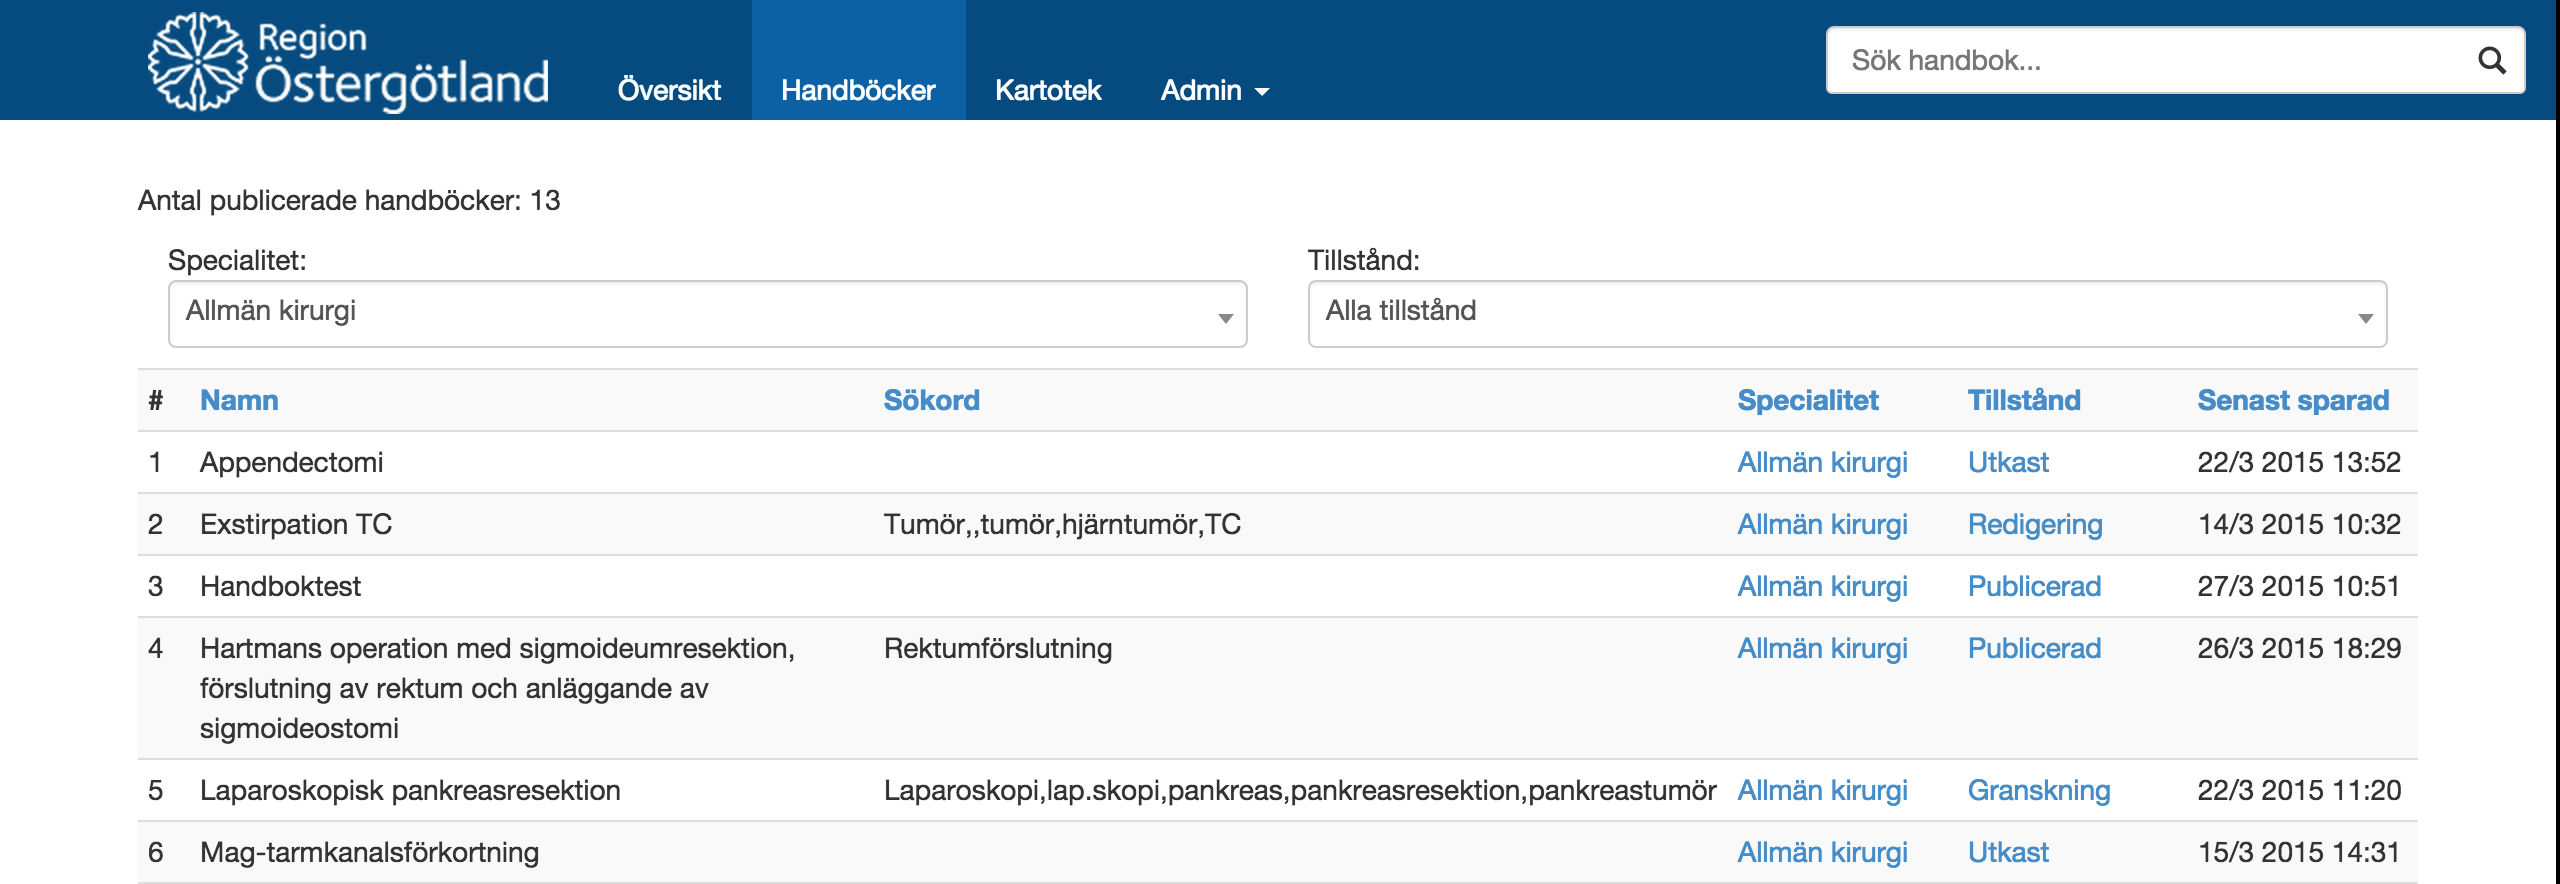
\includegraphics[width=0.6\textwidth]{images/site/list}
  \caption{Lista med handböcker}
  \label{fig:list}
\end{figure}

\subsubsection{Administrering}
I administreringsvyn kan man utöver att redigera all information även sortera processer och rubriker genom att dra och släppa dem.
Redigeringen under rubrikerna använder sig av en wysiwyg-editor.
Innan en redigerad eller ny handbok publiceras måste den granskas av en annan person.

\subsubsection{Operationsförberedelse}
En operationsförberedelse är nästan likadan som en handbok.
Det som skiljer är att vissa av rubrikerna kan gå att kryssa av när de är klara.

\begin{figure}
  \centering
  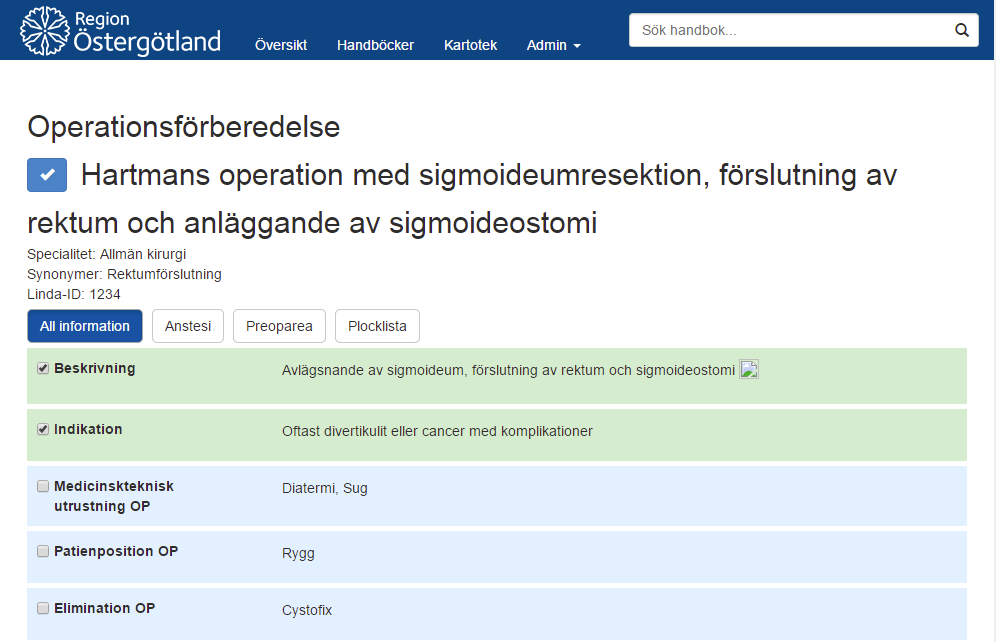
\includegraphics[width=0.6\textwidth]{images/site/op}
  \caption{Förberedelsevyn}
  \label{fig:op}
\end{figure}

I figur \ref{fig:op} kan man se att rubrikerna går att kryssa av när de är klara. Jämför med figur \ref{fig:handbok} där rubrikerna inte går att kryssa av.

\subsubsection{Plocklista}
En operationsförberedelse har även en plocklista med artiklar som behövs till operationen.

\begin{figure}
  \centering
  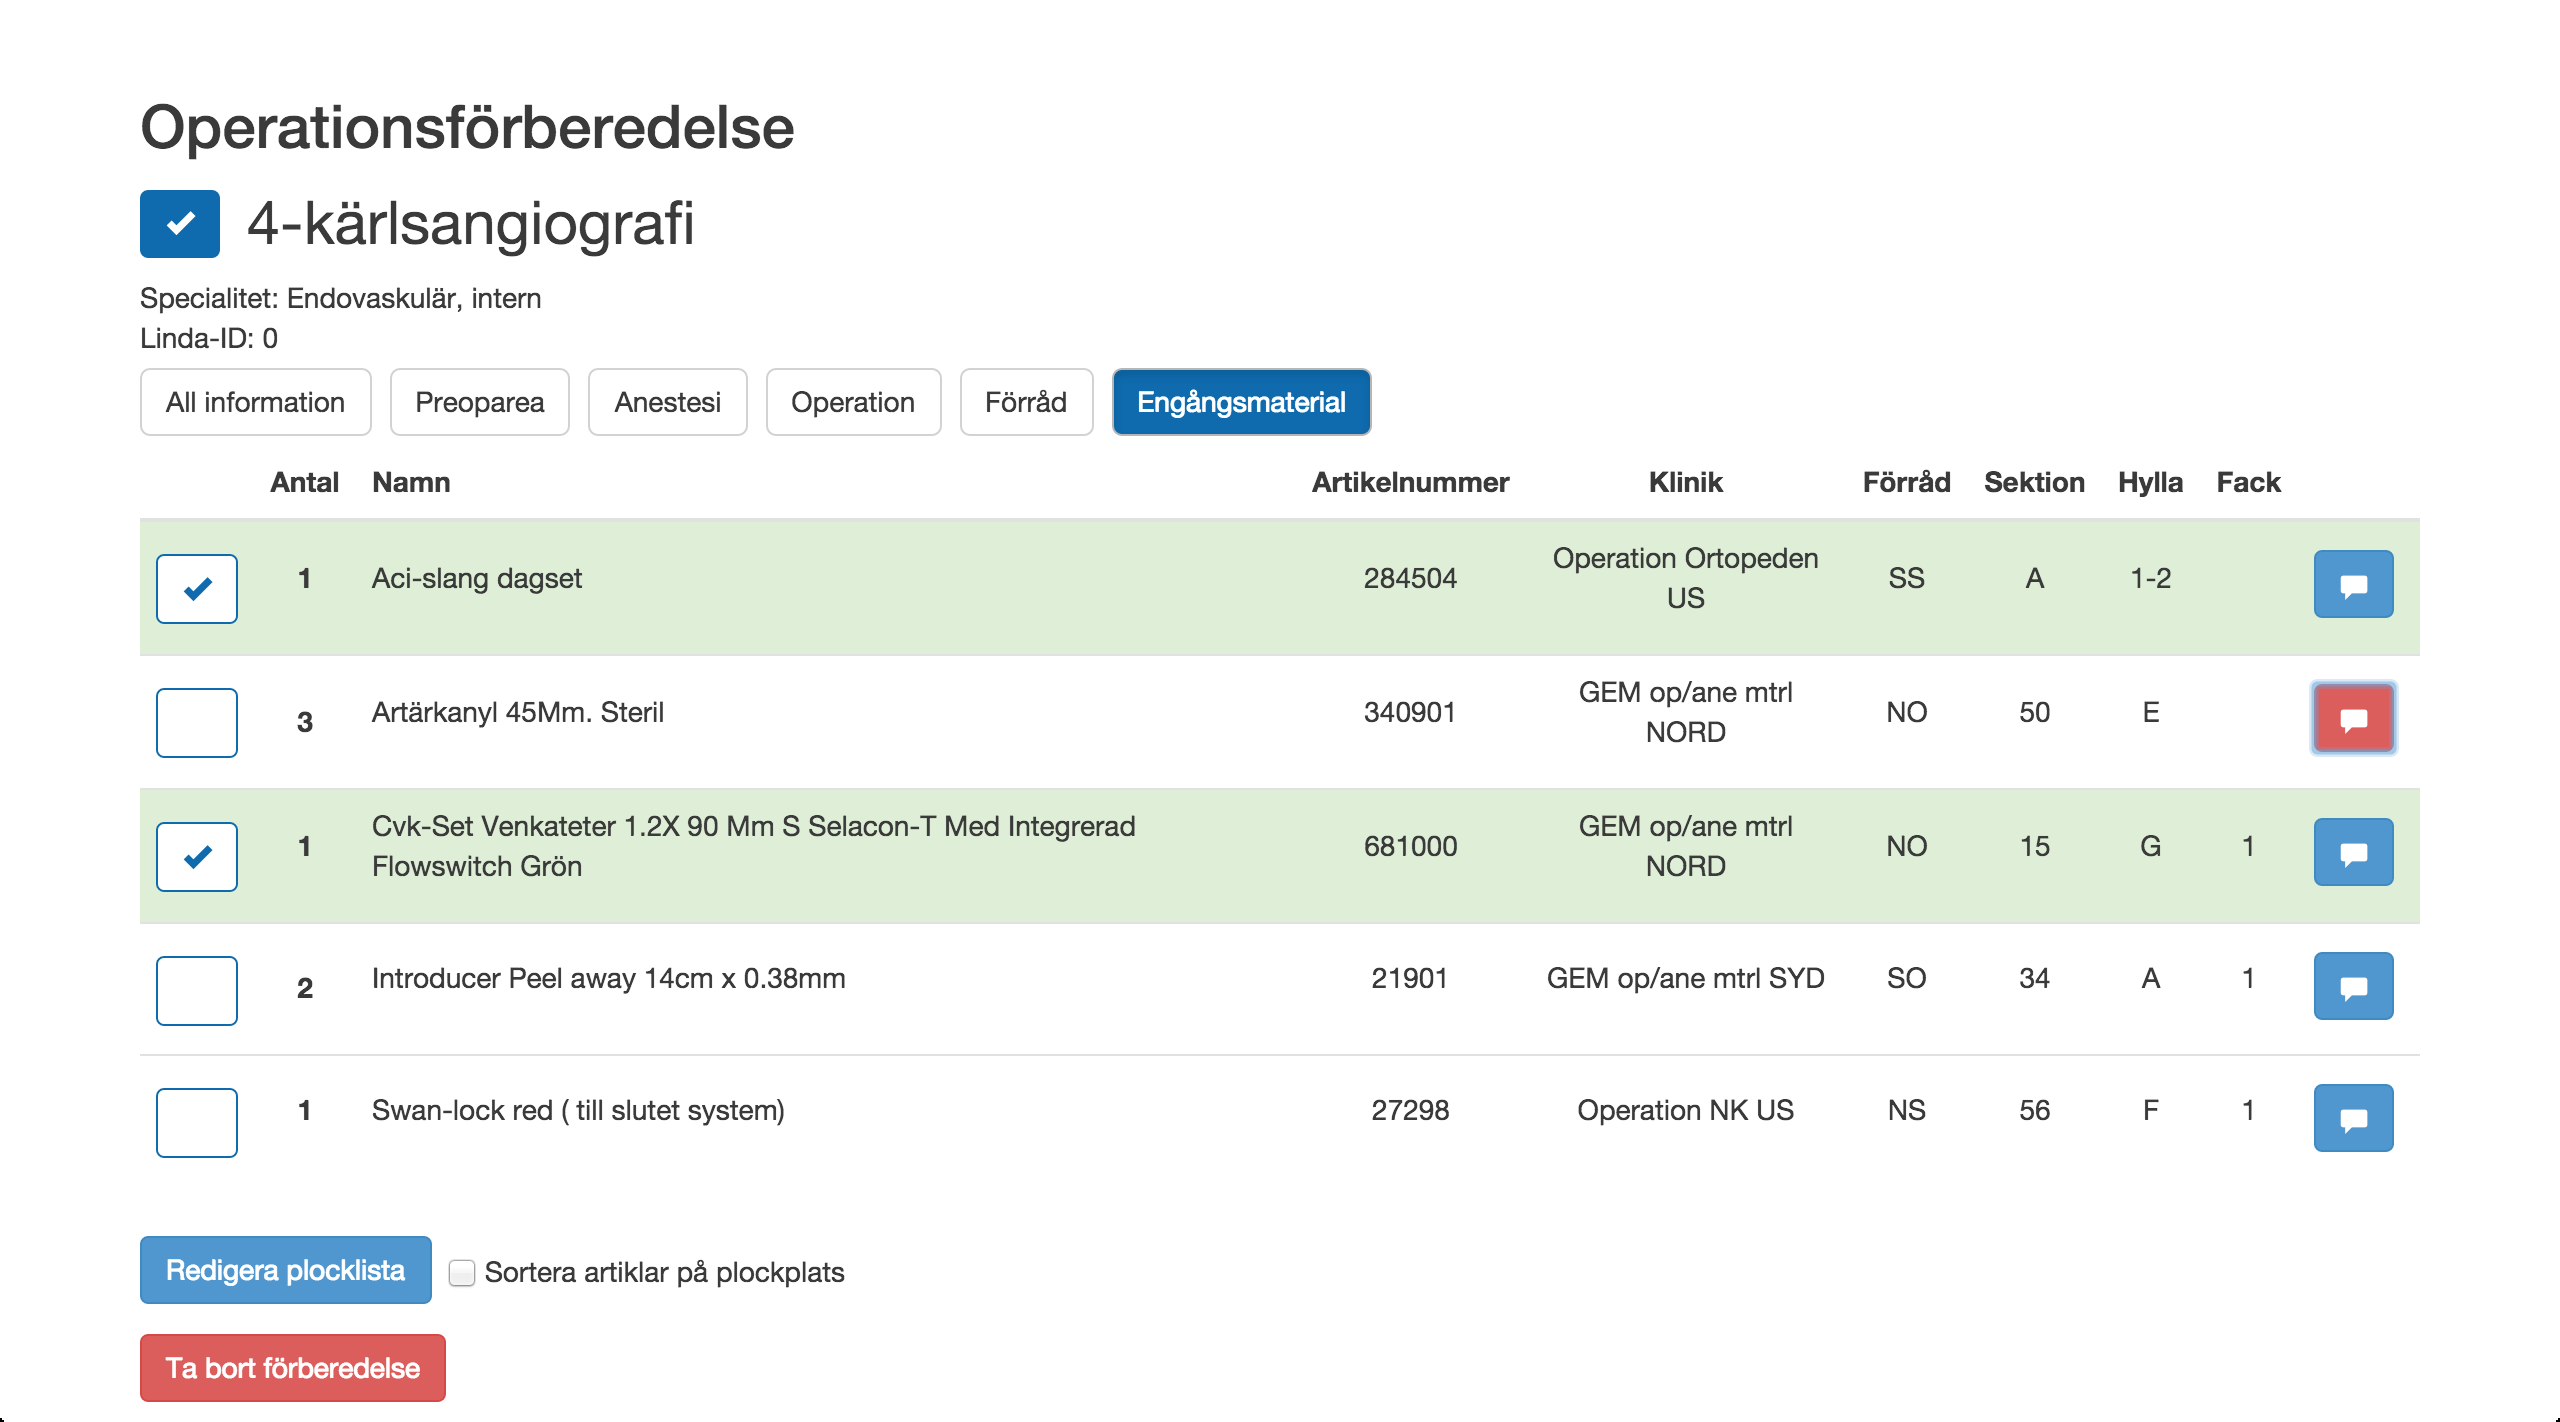
\includegraphics[width=0.6\textwidth]{images/site/plocklista}
  \caption{Plocklista}
  \label{fig:plocklista}
\end{figure}

I figur \ref{fig:plocklista} kan man även se att det finns stöd för att lägga en kommentar på en artikel.
Det är vanligt att en artikel är slut eller utbytt och man kan då lägga en kommentar på varför man inte kunde hämta den artikeln och även hur man har löst det istället.

\subsubsection{Kartoteket}
Kartoteket diskuteras i djup detalj nedan.

\subsection{Utvecklingen}
Här nedan beskrivs resultatet av hur utvecklingen inom gruppen har fungerat, och huruvida de olika hjälpmedlen har hjälpt eller stjälpt.

\subsubsection{SCRUM}
Utvecklingen i SCRUM-form har fungerat bra, dock har utvecklingen som beskriven i metod inte varit i rent SCRUM-format utan har modifierats för att bättre passa gruppen. Ett möte med handledare har hållits en gång i veckan där handledaren har haft möjlighet att ta upp saker som denne tyckt har behövts, sedan har gruppen hållit ett kort SCRUM-möte där man fått förklara vad man gjort förra veckan och vad man planerat att göra kommande vecka. Under mötets gång har man noterat om det är någonting som har behövt diskuteras vidare och detta har då noterats, varpå gruppen har gått igenom dessa frågor efteråt. Detta har fungerat väldigt bra då man på detta sättet inte har fått några större avbrott och alla hela tiden kunna hålla fokus. Efter SCRUM-mötena så har ordet varit fritt och alla har haft möjligheten att komma med synpunkter eller åsikter över någonting.

\subsubsection{Alpha state cards}
Korten har kontinuerligt uppdaterats av teamledare, dock har de kanske inte använts lika flitigt av gruppen som tanken var att de skulle?

\subsubsection{Kundmöten}
I inledningen av projektet hölls några längre kundmöten \textbf{HUR MÅNGA, OCH VAD DISKUTERADES?}, där endast teamledaren, kundansvarige och arkitekten närvarade från projektgruppen. Detta möte hölls främst för att kunden skulle få framföra sina önskemål. Sedan gjordes ett studiebesök hos kund där alla gruppmedlemmar deltog. Man fick se hur en sjuksköterska förberedde inför en operation och även se deras nuvarande system i bruk.

Efter varje iteration hölls ett möte på plats hos kunden för att diskutera hur arbetet fortskred, detta var även ett perfekt tillfälle att ta upp saker man var osäker kring, men var även bra för båda parter att föreslå ändringar.

\subsubsection{Samarbete i gruppen}
Samarbetet i gruppen har fungerat väldigt bra, kodstugorna som gruppen höll under förstudien fungerade riktigt bra och de som var mindre erfarna med webbprogrammering kände att de fick all den hjälp de behövde när de körde fast i sitt arbete och därför kändes det naturligt för hela gruppen att fortsätta med dessa även under utvecklingsfasen.

%\subsection{Gruppens gemensamma erfarenheter}
%\subsection{Översikt över de inviduella utredningarna}
